%\VignetteIndexEntry{metagenomeSeq: statistical analysis for sparse high-throughput sequencing}
%\VignetteEngine{knitr::knitr}
\documentclass[a4paper,11pt]{article}\usepackage[]{graphicx}\usepackage[]{color}
%% maxwidth is the original width if it is less than linewidth
%% otherwise use linewidth (to make sure the graphics do not exceed the margin)
\makeatletter
\def\maxwidth{ %
  \ifdim\Gin@nat@width>\linewidth
    \linewidth
  \else
    \Gin@nat@width
  \fi
}
\makeatother

\definecolor{fgcolor}{rgb}{0.345, 0.345, 0.345}
\newcommand{\hlnum}[1]{\textcolor[rgb]{0.686,0.059,0.569}{#1}}%
\newcommand{\hlstr}[1]{\textcolor[rgb]{0.192,0.494,0.8}{#1}}%
\newcommand{\hlcom}[1]{\textcolor[rgb]{0.678,0.584,0.686}{\textit{#1}}}%
\newcommand{\hlopt}[1]{\textcolor[rgb]{0,0,0}{#1}}%
\newcommand{\hlstd}[1]{\textcolor[rgb]{0.345,0.345,0.345}{#1}}%
\newcommand{\hlkwa}[1]{\textcolor[rgb]{0.161,0.373,0.58}{\textbf{#1}}}%
\newcommand{\hlkwb}[1]{\textcolor[rgb]{0.69,0.353,0.396}{#1}}%
\newcommand{\hlkwc}[1]{\textcolor[rgb]{0.333,0.667,0.333}{#1}}%
\newcommand{\hlkwd}[1]{\textcolor[rgb]{0.737,0.353,0.396}{\textbf{#1}}}%

\usepackage{framed}
\makeatletter
\newenvironment{kframe}{%
 \def\at@end@of@kframe{}%
 \ifinner\ifhmode%
  \def\at@end@of@kframe{\end{minipage}}%
  \begin{minipage}{\columnwidth}%
 \fi\fi%
 \def\FrameCommand##1{\hskip\@totalleftmargin \hskip-\fboxsep
 \colorbox{shadecolor}{##1}\hskip-\fboxsep
     % There is no \\@totalrightmargin, so:
     \hskip-\linewidth \hskip-\@totalleftmargin \hskip\columnwidth}%
 \MakeFramed {\advance\hsize-\width
   \@totalleftmargin\z@ \linewidth\hsize
   \@setminipage}}%
 {\par\unskip\endMakeFramed%
 \at@end@of@kframe}
\makeatother

\definecolor{shadecolor}{rgb}{.97, .97, .97}
\definecolor{messagecolor}{rgb}{0, 0, 0}
\definecolor{warningcolor}{rgb}{1, 0, 1}
\definecolor{errorcolor}{rgb}{1, 0, 0}
\newenvironment{knitrout}{}{} % an empty environment to be redefined in TeX

\usepackage{alltt}
\usepackage{url}
\usepackage{afterpage}
\usepackage{hyperref}
\usepackage{geometry}
\usepackage{cite}
\geometry{hmargin=2.5cm, vmargin=2.5cm}
\usepackage{graphicx}
\usepackage{courier}
\bibliographystyle{unsrt}
\IfFileExists{upquote.sty}{\usepackage{upquote}}{}

\begin{document}



\title{{\textbf{\texttt{metagenomeSeq}: Statistical analysis for sparse high-throughput sequencing}}}
\author{Joseph Nathaniel Paulson\\[1em]\\ Applied Mathematics $\&$ Statistics, and Scientific Computation\\ Center for Bioinformatics and Computational Biology\\ University of Maryland, College Park\\[1em]\\ \texttt{jpaulson@umiacs.umd.edu}}
\date{Modified: November 19, 2013. Compiled: \today}
\maketitle
\tableofcontents

\newpage




\section{Introduction}
\textbf{This is a vignette for pieces of an association study pipeline. For a full list of functions available in the package: help(package=metagenomeSeq). For more information about a particular function call: ?function.}

Metagenomics is the study of genetic material targeted directly from an environmental community. 
Originally focused on exploratory and validation projects, these studies now focus on understanding the differences in microbial communities caused by phenotypic differences. 
Analyzing high-throughput sequencing data has been a challenge to researchers due to the unique biological and technological biases that are present in marker-gene survey data.

 We present a R package, \texttt{metagenomeSeq}, that implements methods developed to account for previously unaddressed biases specific to high-throughput sequencing microbial marker-gene survey data. Our method implements a novel normalization technique and method to account for sparsity due to undersampling. Other methods include
 White \textit{et al.}'s Metastats and Segata \textit{et al.}'s LEfSe. The first is a non-parametric permutation test on $t$-statistics and the second is a non-parametric Kruskal-Wallis test followed by subsequent wilcox rank-sum tests on subgroups to guard against positive discoveries of differential abundance driven by potential confounders - neither address normalization nor sparsity.

This vignette describes the basic protocol when using \texttt{metagenomeSeq}. 
A normalization method able to control for biases in measurements across taxanomic features and a mixture model that implements a zero-inflated Gaussian distribution to account for varying depths of coverage are implemented.
Using a linear model methodology, it is easy to include confounding sources of variability and interpret results. 
Additionally, visualization functions are provided to examine discoveries. 

The software was designed to determine features (be it Operational Taxanomic Unit (OTU), species, etc.) that are differentially abundant between two or more groups of multiple samples. 
The software was also designed to address the effects of both normalization and undersampling of microbial communities on disease association detection and testing of feature correlations.

\begin{figure}
\centerline{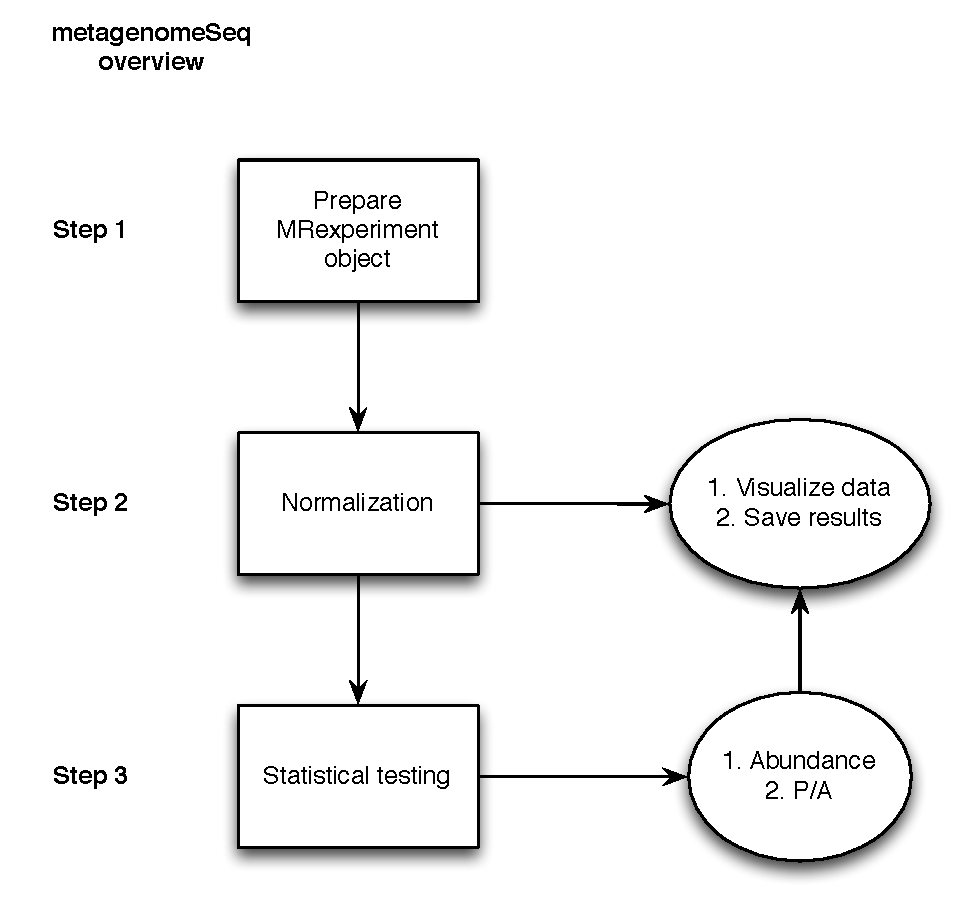
\includegraphics[width=.55\textwidth]{overview.pdf}}
\caption{General overview. metagenomeSeq requires the user to convert their data into MRexperiment objects. Using those MRexperiment objects, one can normalize their data, run statistical tests (abundance or presence-absence), and visualize or save results.}
\end{figure}

\newpage
\section{Data preparation}
Microbial marker gene sequence data is preprocessed and counts are algorithmically defined 
from project-specific sequence data by clustering reads according to read similarity. 
Given $m$ features and $n$ samples, the elements in a count matrix 
\textbf{C} ($m, n$), $c_{ij}$, are the number of reads annotated for a particular 
feature $i$ (whether it be OTU, species, genus, etc.) in sample $j$. \\


\begin{center}
$\bordermatrix{ &sample_1&sample_2&\ldots &sample_n\cr feature_1&c_{11} &  c_{12}  & \ldots & c_{1n}\cr feature_2& c_{21}  &  c_{22} & \ldots & c_{2n}\cr \vdots & \vdots & \vdots & \ddots & \vdots\cr feature_m & c_{m1}  &   c_{m2} &\ldots & c_{mn}}$
\end{center}

Count data should be stored in a delimited (tab by default) file with sample names
along the first row and feature names along the first column.

Data is prepared and formatted as a MRexperiment object. For an overview of the internal structure please see Appendix A.

\subsection{Example datasets}
There are two datasets included as examples in the \texttt{metagenomeSeq} package. Data needs to be in a \texttt{MRexperiment} object format to normalize, run statistical tests, and visualize. As an example, throughout the vignette we'll use the following datasets. 
To understand a function's usage or included data simply enter ?functionName.

\begin{knitrout}
\definecolor{shadecolor}{rgb}{0.969, 0.969, 0.969}\color{fgcolor}\begin{kframe}
\begin{alltt}
\hlkwd{library}\hlstd{(metagenomeSeq)}
\end{alltt}
\end{kframe}
\end{knitrout}


\begin{enumerate}
\item Human lung microbiome \cite{charlson}:
The lung microbiome consists of respiratory flora sampled from six healthy individuals. Three healthy nonsmokers and three healthy smokers. The upper lung tracts were sampled by oral wash and oro-/nasopharyngeal swabs. Samples were taken using two bronchoscopes, serial bronchoalveolar lavage and lower airway protected brushes.
\end{enumerate}
\begin{knitrout}
\definecolor{shadecolor}{rgb}{0.969, 0.969, 0.969}\color{fgcolor}\begin{kframe}
\begin{alltt}
\hlkwd{data}\hlstd{(lungData)}
\hlstd{lungData}
\end{alltt}
\begin{verbatim}
## MRexperiment (storageMode: environment)
## assayData: 51891 features, 78 samples 
##   element names: counts 
## protocolData: none
## phenoData
##   sampleNames: CHK_6467_E3B11_BRONCH2_PREWASH_V1V2
##     CHK_6467_E3B11_OW_V1V2 ... CHK_6467_E3B09_BAL_A_V1V2
##     (78 total)
##   varLabels: SampleType SiteSampled SmokingStatus
##   varMetadata: labelDescription
## featureData
##   featureNames: 1 2 ... 51891 (51891 total)
##   fvarLabels: taxa
##   fvarMetadata: labelDescription
## experimentData: use 'experimentData(object)'
##   pubMedIds: 21680950 
## Annotation:
\end{verbatim}
\end{kframe}
\end{knitrout}


\begin{enumerate}
\setcounter{enumi}{1}
\item Humanized gnotobiotic mouse gut \cite{ts_mouse}:
Twelve germ-free adult male C57BL/6J mice were fed a low-fat, plant polysaccharide-rich diet. Each mouse was gavaged with healthy adult human fecal material. Following the fecal transplant, mice remained on the low-fat, plant polysacchaaride-rich diet for four weeks, following which a subset of 6 were switched to a high-fat and high-sugar diet for eight weeks. Fecal samples for each mouse went through PCR amplification of the bacterial 16S rRNA gene V2 region weekly. Details of experimental protocols and further details of the data can be found in Turnbaugh et. al. Sequences and further information can be found at:
\url{http://gordonlab.wustl.edu/TurnbaughSE_10_09/STM_2009.html}

\end{enumerate}
\begin{knitrout}
\definecolor{shadecolor}{rgb}{0.969, 0.969, 0.969}\color{fgcolor}\begin{kframe}
\begin{alltt}
\hlkwd{data}\hlstd{(mouseData)}
\hlstd{mouseData}
\end{alltt}
\begin{verbatim}
## MRexperiment (storageMode: environment)
## assayData: 10172 features, 139 samples 
##   element names: counts 
## protocolData: none
## phenoData
##   sampleNames: PM1:20080107 PM1:20080108 ... PM9:20080303
##     (139 total)
##   varLabels: mouseID date diet
##   varMetadata: labelDescription
## featureData
##   featureNames: Prevotellaceae:1 Lachnospiraceae:1 ...
##     Parabacteroides:956 (10172 total)
##   fvarLabels: fdata
##   fvarMetadata: labelDescription
## experimentData: use 'experimentData(object)'
##   pubMedIds: 20368178 
## Annotation:
\end{verbatim}
\end{kframe}
\end{knitrout}


\subsection{Loading count data}
Following preprocessing and annotation of sequencing data \texttt{metagenomeSeq} requires a count matrix with features along rows and samples along the columns.
\texttt{metagenomeSeq} includes functions for loading delimited files of counts 
\texttt{load$\_$meta} and phenodata \texttt{load$\_$phenoData}.

As an example, a portion of the lung microbiome \cite{charlson} 
OTU matrix is provided in \texttt{metagenomeSeq}'s library "extdata" folder. 
The OTU matrix is stored as a tab delimited file.
\texttt{load\_meta} loads the taxa and counts into a list.

\begin{knitrout}
\definecolor{shadecolor}{rgb}{0.969, 0.969, 0.969}\color{fgcolor}\begin{kframe}
\begin{alltt}
\hlstd{dataDirectory} \hlkwb{<-} \hlkwd{system.file}\hlstd{(}\hlstr{"extdata"}\hlstd{,} \hlkwc{package} \hlstd{=} \hlstr{"metagenomeSeq"}\hlstd{)}
\hlstd{lung} \hlkwb{=} \hlkwd{load_meta}\hlstd{(}\hlkwd{file.path}\hlstd{(dataDirectory,} \hlstr{"CHK_NAME.otus.count.csv"}\hlstd{))}
\hlkwd{dim}\hlstd{(lung}\hlopt{$}\hlstd{counts)}
\end{alltt}
\begin{verbatim}
## [1] 1000   78
\end{verbatim}
\end{kframe}
\end{knitrout}



\subsection{Loading taxonomy}
Next we want to load the annotated taxonomy. Check to make sure that your taxa annotations and OTUs are in the same order as your matrix rows.

\begin{knitrout}
\definecolor{shadecolor}{rgb}{0.969, 0.969, 0.969}\color{fgcolor}\begin{kframe}
\begin{alltt}
\hlstd{taxa} \hlkwb{=} \hlkwd{read.delim}\hlstd{(}\hlkwd{file.path}\hlstd{(dataDirectory,} \hlstr{"CHK_otus.taxonomy.csv"}\hlstd{),}
    \hlkwc{stringsAsFactors} \hlstd{= F)[,} \hlnum{2}\hlstd{]}
\hlstd{otu} \hlkwb{=} \hlkwd{read.delim}\hlstd{(}\hlkwd{file.path}\hlstd{(dataDirectory,} \hlstr{"CHK_otus.taxonomy.csv"}\hlstd{),}
    \hlkwc{stringsAsFactors} \hlstd{= F)[,} \hlnum{1}\hlstd{]}
\end{alltt}
\end{kframe}
\end{knitrout}



As our OTUs appear to be in order with the count matrix we loaded earlier, the next step is to load phenodata. 

\textbf{Warning}: features need to have the same names as the rows of the count matrix when we create the MRexperiment object for provenance purposes. 

\subsection{Loading metadata}
Phenotype data can be optionally loaded into \texttt{R} with \texttt{load\_phenoData}. This function loads the data as a list.

\begin{knitrout}
\definecolor{shadecolor}{rgb}{0.969, 0.969, 0.969}\color{fgcolor}\begin{kframe}
\begin{alltt}
\hlstd{clin} \hlkwb{=} \hlkwd{load_phenoData}\hlstd{(}\hlkwd{file.path}\hlstd{(dataDirectory,} \hlstr{"CHK_clinical.csv"}\hlstd{),}
    \hlkwc{tran} \hlstd{=} \hlnum{TRUE}\hlstd{)}
\hlstd{ord} \hlkwb{=} \hlkwd{match}\hlstd{(}\hlkwd{colnames}\hlstd{(lung}\hlopt{$}\hlstd{counts),} \hlkwd{rownames}\hlstd{(clin))}
\hlstd{clin} \hlkwb{=} \hlstd{clin[ord, ]}
\hlkwd{head}\hlstd{(clin[}\hlnum{1}\hlopt{:}\hlnum{2}\hlstd{, ])}
\end{alltt}
\begin{verbatim}
##                                          SampleType
## CHK_6467_E3B11_BRONCH2_PREWASH_V1V2 Bronch2.PreWash
## CHK_6467_E3B11_OW_V1V2                           OW
##                                              SiteSampled
## CHK_6467_E3B11_BRONCH2_PREWASH_V1V2 Bronchoscope.Channel
## CHK_6467_E3B11_OW_V1V2                        OralCavity
##                                     SmokingStatus
## CHK_6467_E3B11_BRONCH2_PREWASH_V1V2        Smoker
## CHK_6467_E3B11_OW_V1V2                     Smoker
\end{verbatim}
\end{kframe}
\end{knitrout}



\textbf{Warning}: phenotypes must have the same names as the columns on the count matrix when we create the MRexperiment object for provenance purposes. 

\subsection{Creating a \texttt{MRexperiment} object}

Function \texttt{newMRexperiment} takes a count matrix, phenoData (annotated data frame), and featureData (annotated data frame) as input. 
\texttt{Biobase} provides functions to create annotated data frames. 
Library sizes (depths of coverage) and normalization factors are also optional inputs.


\begin{knitrout}
\definecolor{shadecolor}{rgb}{0.969, 0.969, 0.969}\color{fgcolor}\begin{kframe}
\begin{alltt}
\hlstd{phenotypeData} \hlkwb{=} \hlkwd{as}\hlstd{(clin,} \hlstr{"AnnotatedDataFrame"}\hlstd{)}
\hlstd{phenotypeData}
\end{alltt}
\begin{verbatim}
## An object of class 'AnnotatedDataFrame'
##   rowNames: CHK_6467_E3B11_BRONCH2_PREWASH_V1V2
##     CHK_6467_E3B11_OW_V1V2 ... CHK_6467_E3B09_BAL_A_V1V2
##     (78 total)
##   varLabels: SampleType SiteSampled SmokingStatus
##   varMetadata: labelDescription
\end{verbatim}
\end{kframe}
\end{knitrout}


A feature annotated data frame. In this example it is simply the OTU numbers, but it can as easily be the annotated taxonomy at multiple levels.

\begin{knitrout}
\definecolor{shadecolor}{rgb}{0.969, 0.969, 0.969}\color{fgcolor}\begin{kframe}
\begin{alltt}
\hlstd{OTUdata} \hlkwb{=} \hlkwd{as}\hlstd{(lung}\hlopt{$}\hlstd{taxa,} \hlstr{"AnnotatedDataFrame"}\hlstd{)}
\hlkwd{varLabels}\hlstd{(OTUdata)} \hlkwb{=} \hlstr{"taxa"}
\hlstd{OTUdata}
\end{alltt}
\begin{verbatim}
## An object of class 'AnnotatedDataFrame'
##   rowNames: 1 2 ... 1000 (1000 total)
##   varLabels: taxa
##   varMetadata: labelDescription
\end{verbatim}
\end{kframe}
\end{knitrout}



\begin{knitrout}
\definecolor{shadecolor}{rgb}{0.969, 0.969, 0.969}\color{fgcolor}\begin{kframe}
\begin{alltt}
\hlstd{obj} \hlkwb{=} \hlkwd{newMRexperiment}\hlstd{(lung}\hlopt{$}\hlstd{counts,}\hlkwc{phenoData}\hlstd{=phenotypeData,}\hlkwc{featureData}\hlstd{=OTUdata)}
\hlcom{# Links to a paper providing further details can be included optionally.}
\hlcom{# experimentData(obj) = annotate::pmid2MIAME("21680950")}
\hlstd{obj}
\end{alltt}
\begin{verbatim}
## MRexperiment (storageMode: environment)
## assayData: 1000 features, 78 samples 
##   element names: counts 
## protocolData: none
## phenoData
##   sampleNames: CHK_6467_E3B11_BRONCH2_PREWASH_V1V2
##     CHK_6467_E3B11_OW_V1V2 ... CHK_6467_E3B09_BAL_A_V1V2
##     (78 total)
##   varLabels: SampleType SiteSampled SmokingStatus
##   varMetadata: labelDescription
## featureData
##   featureNames: 1 2 ... 1000 (1000 total)
##   fvarLabels: taxa
##   fvarMetadata: labelDescription
## experimentData: use 'experimentData(object)'
## Annotation:
\end{verbatim}
\end{kframe}
\end{knitrout}


Alternatively, you can load in Biome-format data (outputs of QIIME and Mothur) using the \texttt{load$\_$biom} function. If a biom class object is already loaded into R it can be converted to a MRexperiment-class object using the \texttt{biom2MRexperiment} function.

\newpage
\section{Normalization}
Normalization is required due to varying depths of coverage across samples. \texttt{cumNorm} is a normalization method that calculates scaling factors equal to the sum of counts up to a particular quantile.

Denote the $l$th quantile of sample $j$ as $q_j^l$, that is, in sample $j$ there are $l$ taxonomic features with counts smaller than $q_j^l$. For $l= \lfloor .95m \rfloor$ then $q_j^l$ corresponds to the 95th percentile of the count distribution for sample $j$. 


Denote $s_j^l= \sum_{(i|c_{ij}\leq q_j^l)}c_{ij}$  as the sum of counts for sample $j$ up to the $l$th quantile. Our normalization chooses a value  $\hat{l}\leq m$ to define a normalization scaling factor for each sample to produce normalized counts $\tilde{c_{ij}}$  = $\frac{c_{ij}}{s_j^{\hat{l}}}N$ where $N$ is an appropriately chosen normalization constant. See Appendix C for more information on how our method calculates the proper percentile.

These normalization factors are stored in the experiment summary slot. Functions to determine the proper percentile \texttt{cumNormStat}, save normalized counts \texttt{exportMat}, or save various sample statistics \texttt{exportStats} are also provided.
Normalized counts can be called easily by \texttt{cumNormMat(MRexperimentObject)} or \texttt{MRcounts(MRexperimentObject,norm=TRUE,log=FALSE)}.

\subsection{Calculating normalization factors}
After defining a \texttt{MRexperiment} object, the first step is to calculate the proper percentile by which to normalize counts. There are several options in calculating and visualizing the relative differences in the reference. Figure 3 is an example from the lung dataset.

\begin{knitrout}
\definecolor{shadecolor}{rgb}{0.969, 0.969, 0.969}\color{fgcolor}\begin{kframe}
\begin{alltt}
\hlkwd{data}\hlstd{(lungData)}
\hlstd{p} \hlkwb{=} \hlkwd{cumNormStatFast}\hlstd{(lungData)}
\end{alltt}
\end{kframe}
\end{knitrout}


\noindent
To calculate the scaling factors we simply run \texttt{cumNorm}

\begin{knitrout}
\definecolor{shadecolor}{rgb}{0.969, 0.969, 0.969}\color{fgcolor}\begin{kframe}
\begin{alltt}
\hlstd{lungData} \hlkwb{=} \hlkwd{cumNorm}\hlstd{(lungData,} \hlkwc{p} \hlstd{= p)}
\end{alltt}
\end{kframe}
\end{knitrout}


The user can alternatively choose different percentiles for the normalization scheme by specifying $p$.

There are other functions, including \texttt{normFactors}, \texttt{cumNormMat}, that return the normalization factors or a normalized matrix for a specified percentile. To see a full list of functions please refer to the manual and help pages. 

\subsection{Exporting data}
To export normalized count matrices:
\begin{knitrout}
\definecolor{shadecolor}{rgb}{0.969, 0.969, 0.969}\color{fgcolor}\begin{kframe}
\begin{alltt}
\hlstd{mat} \hlkwb{=} \hlkwd{MRcounts}\hlstd{(lungData,} \hlkwc{norm} \hlstd{=} \hlnum{TRUE}\hlstd{,} \hlkwc{log} \hlstd{=} \hlnum{TRUE}\hlstd{)[}\hlnum{1}\hlopt{:}\hlnum{5}\hlstd{,} \hlnum{1}\hlopt{:}\hlnum{5}\hlstd{]}
\hlkwd{exportMat}\hlstd{(mat,} \hlkwc{output} \hlstd{=} \hlkwd{file.path}\hlstd{(dataDirectory,} \hlstr{"tmp.tsv"}\hlstd{))}
\end{alltt}
\end{kframe}
\end{knitrout}


\noindent
To save sample statistics (sample scaling factor, quantile value, number of identified features and library size):
\begin{knitrout}
\definecolor{shadecolor}{rgb}{0.969, 0.969, 0.969}\color{fgcolor}\begin{kframe}
\begin{alltt}
\hlkwd{exportStats}\hlstd{(lungData[,} \hlnum{1}\hlopt{:}\hlnum{5}\hlstd{],} \hlkwc{output} \hlstd{=} \hlkwd{file.path}\hlstd{(dataDirectory,} \hlstr{"tmp.tsv"}\hlstd{))}
\hlkwd{head}\hlstd{(}\hlkwd{read.csv}\hlstd{(}\hlkwc{file} \hlstd{=} \hlkwd{file.path}\hlstd{(dataDirectory,} \hlstr{"tmp.tsv"}\hlstd{),} \hlkwc{sep} \hlstd{=} \hlstr{"\textbackslash{}t"}\hlstd{))}
\end{alltt}
\begin{verbatim}
##                               Subject Scaling.factor
## 1 CHK_6467_E3B11_BRONCH2_PREWASH_V1V2             67
## 2              CHK_6467_E3B11_OW_V1V2           2475
## 3              CHK_6467_E3B08_OW_V1V2           2198
## 4           CHK_6467_E3B07_BAL_A_V1V2            836
## 5           CHK_6467_E3B11_BAL_A_V1V2           1008
##   Quantile.value Number.of.identified.features Library.size
## 1              1                            60          271
## 2              1                          3299         7863
## 3              1                          2994         8360
## 4              1                          1188         5249
## 5              1                          1098         3383
\end{verbatim}
\end{kframe}
\end{knitrout}






\newpage
\section{Statistical testing}
Now that we have taken care of normalization we can address the effects of under sampling on the detecting differentially abundant features (OTUs, genes, etc).

\subsection{Zero-inflated Gaussian mixture model}
The depth of coverage in a sample is directly related to how many features are detected in a sample motivating our zero-inflated Gaussian (ZIG) mixture model. Figure 2 is representative of the linear relationship between depth of coverage and OTU identification ubiquitous in marker-gene survey datasets currently available. For a quick overview of the mathematical model see Appendix B.

\begin{figure}
\centerline{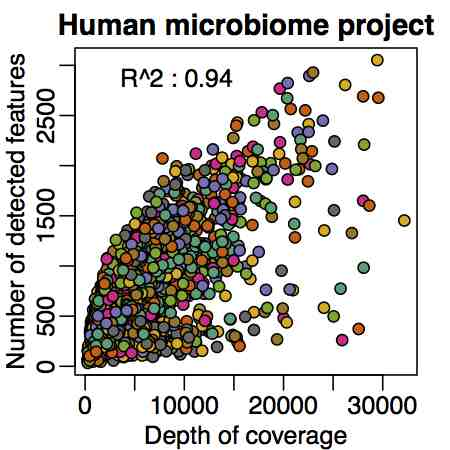
\includegraphics[width=.55\textwidth]{metagenomeSeq_figure1.png}}
\caption{\footnotesize{The number of unique features is plotted against depth of coverage for samples from the Human Microbiome Project \cite{hmp}. Including the depth of coverage and the interaction of body site and sequencing site we are able to acheive an adjusted $\mathrm{R}^2$ of .94. The zero-inflated Gaussian mixture was developed to account for missing features.}}\label{fig1}
\end{figure}

Function \texttt{fitZig} performs a complex mathematical optimization routine to estimate probabilities that a zero for a particular feature in a sample is a technical zero or not. The function relies heavily on the \texttt{limma} package \cite{limma}. Design matrices can be created in R by using the \texttt{model.matrix} function and are inputs for \texttt{fitZig}. 

For large survey studies it is often pertinent to include phenotype information or confounders into a design matrix when testing the association between the abundance of taxonomic features and a phenotype phenotype of interest (disease, for
instance). Our linear model methodology can easily incorporate these
confounding covariates in a straightforward manner. \texttt{fitZig} output includes weighted fits for each of the $m$ features. Results can be filtered and saved using \texttt{MRcoefs} or \texttt{MRtable}.

\subsection{Example using fitZig for differential abundance testing}
\textbf{Warning}: The user should restrict significant features to those with a minimum number of positive samples. What this means is that one should not claim features are significant unless the effective number of samples is above a particular percentage. For example, fold-change estimates might be unreliable if an entire group does not have a positive count for the feature in question.


We recommend the user remove features based on the number of estimated effective samples, please see \texttt{calculateEffectiveSamples}. We recommend removing features with less than the average number of effective samples in all features. In essence, setting eff = .5 when using \texttt{MRcoefs}, \texttt{MRfulltable}, or \texttt{MRtable}.

In our analysis of the lung microbiome data, we can remove features that are not present in many samples, controls, and calculate the normalization factors. The user needs to decide which metadata should be included in the linear model.

\begin{knitrout}
\definecolor{shadecolor}{rgb}{0.969, 0.969, 0.969}\color{fgcolor}\begin{kframe}
\begin{alltt}
\hlstd{controls} \hlkwb{=} \hlkwd{grep}\hlstd{(}\hlstr{"Extraction.Control"}\hlstd{,} \hlkwd{pData}\hlstd{(lungData)}\hlopt{$}\hlstd{SampleType)}
\hlstd{lungTrim} \hlkwb{=} \hlstd{lungData[,} \hlopt{-}\hlstd{controls]}
\hlstd{sparseFeatures} \hlkwb{=} \hlkwd{which}\hlstd{(}\hlkwd{rowSums}\hlstd{(}\hlkwd{MRcounts}\hlstd{(lungTrim)} \hlopt{>} \hlnum{0}\hlstd{)} \hlopt{<} \hlnum{10}\hlstd{)}
\hlstd{lungTrim} \hlkwb{=} \hlstd{lungTrim[}\hlopt{-}\hlstd{sparseFeatures, ]}
\hlstd{lungp} \hlkwb{=} \hlkwd{cumNormStat}\hlstd{(lungTrim,} \hlkwc{pFlag} \hlstd{=} \hlnum{TRUE}\hlstd{,} \hlkwc{main} \hlstd{=} \hlstr{"Trimmed lung data"}\hlstd{)}
\end{alltt}
\end{kframe}\begin{figure}[]


{\centering 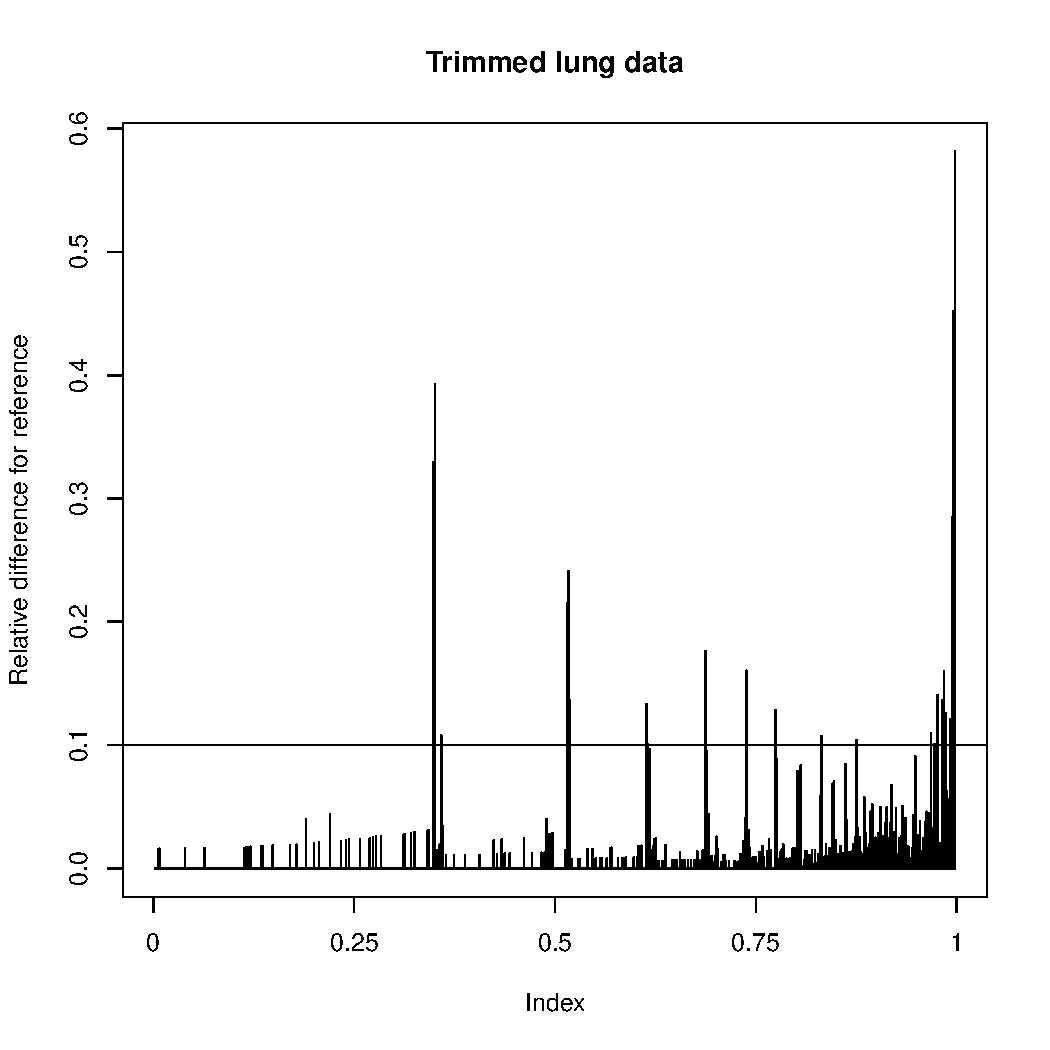
\includegraphics[width=.55\linewidth,height=.55\linewidth]{figure/preprocess} 

}

\caption[Relative difference for the median difference in counts from the reference]{Relative difference for the median difference in counts from the reference.\label{fig:preprocess}}
\end{figure}

\begin{kframe}\begin{alltt}
\hlstd{lungTrim} \hlkwb{=} \hlkwd{cumNorm}\hlstd{(lungTrim,} \hlkwc{p} \hlstd{= lungp)}
\end{alltt}
\end{kframe}
\end{knitrout}


After the user defines an appropriate model matrix for hypothesis testing there are optional inputs to \texttt{fitZig}, including settings determined by \texttt{zigControl}. We ask the user to review the help files for both \texttt{fitZig} and \texttt{zigControl}. For this example we include body site as covariates and want to test for the bacteria differentially abundant between smokers and non-smokers.

\begin{knitrout}
\definecolor{shadecolor}{rgb}{0.969, 0.969, 0.969}\color{fgcolor}\begin{kframe}
\begin{alltt}
\hlstd{smokingStatus} \hlkwb{=} \hlkwd{pData}\hlstd{(lungTrim)}\hlopt{$}\hlstd{SmokingStatus}
\hlstd{bodySite} \hlkwb{=} \hlkwd{pData}\hlstd{(lungTrim)}\hlopt{$}\hlstd{SampleType}
\hlstd{mod} \hlkwb{=} \hlkwd{model.matrix}\hlstd{(}\hlopt{~}\hlstd{smokingStatus} \hlopt{+} \hlstd{bodySite)}
\hlstd{settings} \hlkwb{=} \hlkwd{zigControl}\hlstd{(}\hlkwc{maxit} \hlstd{=} \hlnum{10}\hlstd{,} \hlkwc{verbose} \hlstd{=} \hlnum{TRUE}\hlstd{)}
\hlstd{fit} \hlkwb{=} \hlkwd{fitZig}\hlstd{(}\hlkwc{obj} \hlstd{= lungTrim,} \hlkwc{mod} \hlstd{= mod,} \hlkwc{control} \hlstd{= settings)}
\end{alltt}
\begin{verbatim}
## it= 0, nll=88.55, log10(eps+1)=Inf, stillActive=1029
## it= 1, nll=93.10, log10(eps+1)=0.07, stillActive=299
## it= 2, nll=93.24, log10(eps+1)=0.05, stillActive=130
## it= 3, nll=93.47, log10(eps+1)=0.07, stillActive=31
## it= 4, nll=93.49, log10(eps+1)=0.05, stillActive=15
## it= 5, nll=93.50, log10(eps+1)=0.02, stillActive=9
## it= 6, nll=93.52, log10(eps+1)=0.01, stillActive=5
## it= 7, nll=93.52, log10(eps+1)=0.00, stillActive=2
## it= 8, nll=93.52, log10(eps+1)=0.00, stillActive=1
## it= 9, nll=93.52, log10(eps+1)=0.00, stillActive=0
\end{verbatim}
\end{kframe}
\end{knitrout}


The result, \texttt{fit}, is a list providing detailed estimates of the fits including a 
\texttt{limma} fit in \texttt{fit\$fit} and an \texttt{ebayes} statistical fit in \texttt{fit\$eb}.
This data can be analyzed like any \texttt{limma} fit and in this example, the column of 
the fitted coefficientsrepresents the fold-change for our "smoker" vs. "nonsmoker" analysis. 

Looking at the particular analysis just performed, there appears to be OTUs representing three
\textit{Prevotella}, two \textit{Neisseria}, and a \textit{Porphyromonas} that are differentially
abundant. One should check that similarly annotated OTUs are not equally differentially 
abundant in controls. 

Alternatively, the user can input a model with their own normalization factors including them directly in the model matrix and specifying the option \texttt{useCSSoffset = FALSE} in fitZig.

\subsection{Exporting fits}
Currently functions are being developed to wrap and output results more neatly, but \texttt{MRcoefs}, \texttt{MRtable}, \texttt{MRfulltable} can be used to view coefficient fits and related statistics and export the data with optional output values - see help files to learn how they differ. 

To only consider features that are found in a large percentage of effectively positive (positive samples + the weight of zero counts included in the Gaussian mixture) use the \textbf{eff} option in the \texttt{MRtables}.

\begin{knitrout}
\definecolor{shadecolor}{rgb}{0.969, 0.969, 0.969}\color{fgcolor}\begin{kframe}
\begin{alltt}
\hlstd{taxa} \hlkwb{=} \hlkwd{sapply}\hlstd{(}\hlkwd{strsplit}\hlstd{(}\hlkwd{as.character}\hlstd{(}\hlkwd{fData}\hlstd{(lungTrim)}\hlopt{$}\hlstd{taxa),} \hlkwc{split} \hlstd{=} \hlstr{";"}\hlstd{),}
    \hlkwa{function}\hlstd{(}\hlkwc{i}\hlstd{) \{}
        \hlstd{i[}\hlkwd{length}\hlstd{(i)]}
    \hlstd{\})}
\hlkwd{head}\hlstd{(}\hlkwd{MRcoefs}\hlstd{(fit,} \hlkwc{taxa} \hlstd{= taxa,} \hlkwc{coef} \hlstd{=} \hlnum{2}\hlstd{))}
\end{alltt}
\begin{verbatim}
##                           smokingStatusSmoker    pValue
## Neisseria polysaccharea                -4.130 2.138e-15
## Neisseria meningitidis                 -3.992 2.056e-14
## Prevotella intermedia                  -2.859 9.189e-12
## Prevotella paludivivens                 2.698 6.764e-09
## Porphyromonas sp. UQD 414              -2.696 9.323e-10
## Prevotella sp. DJF_B116                 2.646 1.297e-10
##                           adjPvalue
## Neisseria polysaccharea   1.467e-13
## Neisseria meningitidis    1.113e-12
## Prevotella intermedia     2.781e-10
## Prevotella paludivivens   6.609e-08
## Porphyromonas sp. UQD 414 1.411e-08
## Prevotella sp. DJF_B116   2.696e-09
\end{verbatim}
\end{kframe}
\end{knitrout}


\subsection{Testing presence-absence}
The hypothesis for the implemented presence-absence test is that the proportion/odds of a given feature present is higher/lower among one group of individuals compared to another, and we want to test whether any difference in the proportions observed is significant. We use Fisher's exact test to create a 2x2 contingency table and calculate p-values, odd's ratios, and confidence intervals.  \texttt{fitPA} calculates the presence-absence for each organism and returns a table of p-values, odd's ratios, and confidence intervals. The function will accept either a \texttt{MRexperiment} object or matrix. \texttt{MRfulltable} when sent a result of fitZig will also include the results of \texttt{fitPA}. If there is a desire for a more detailed description, please email me.


\begin{knitrout}
\definecolor{shadecolor}{rgb}{0.969, 0.969, 0.969}\color{fgcolor}\begin{kframe}
\begin{alltt}
\hlkwd{data}\hlstd{(mouseData)}
\hlstd{classes} \hlkwb{=} \hlkwd{pData}\hlstd{(mouseData)}\hlopt{$}\hlstd{diet}
\hlstd{res} \hlkwb{=} \hlkwd{fitPA}\hlstd{(mouseData[}\hlnum{1}\hlopt{:}\hlnum{5}\hlstd{, ],} \hlkwc{cl} \hlstd{= classes)}
\hlcom{# Warning - the p-value is calculating 1 despite a high odd's}
\hlcom{# ratio.}
\hlkwd{head}\hlstd{(res)}
\end{alltt}
\begin{verbatim}
##                         pvalues oddsRatio  lower upper
## Prevotellaceae:1              1       Inf 0.0163   Inf
## Lachnospiraceae:1             1       Inf 0.0163   Inf
## Unclassified-Screened:1       1       Inf 0.0163   Inf
## Clostridiales:1          0.3885         0      0 24.78
## Clostridiales:2               1       Inf 0.0163   Inf
\end{verbatim}
\end{kframe}
\end{knitrout}


\newpage
\section{Aggregating features}
Normalization is recommended at the OTU level. However, functions are in place to aggregate 
the count matrix (normalized or not), based on a particular user defined level. Using the
featureData information in the MRexperiment object, calling \texttt{aggregateByTaxonomy} or \texttt{aggTax} on a MRexperiment object and declaring particular featureData column name (i.e.
'genus') will aggregate counts to the desired level with the aggfun function (default colSums). Possible aggfun alternatives include colMeans and colMedians.


\newpage
\section{Visualization of features}

\texttt{metagenomeSeq} has several plotting functions to visualize and gain insight into the overall structural composition of the 
data. Heatmaps of feature counts: \texttt{plotMRheatmap}. Basic feature correlation structures: \texttt{plotCorr}. PCA/MDS coordinates of 
samples or features: \texttt{plotOrd}. And rarefaction effects: \texttt{plotRare}. 

Other plotting functions include plotting the abundance
differences for a single feature, \texttt{plotOTU} or multiple features
\texttt{plotGenus}. Plotting multiple OTUs with similar annotations allows for
additional control of false discoveries.

\subsection{Structural overview}
Many studies begin by comparing the abundance composition across 
sample or feature phenotypes. Often a first step of data analysis is a 
heatmap, correlation or co-occurence plot or some other data exploratory method. 
The following functions have been implemented to provide a first step overview 
of the data:


\begin{enumerate}
\item \texttt{plotMRheatmap} - heatmap of abundance estimates (Fig. 4 right)
\item \texttt{plotCorr} - heatmap of pairwise correlations (Fig. 4 left)
\item \texttt{plotOrd} - PCA/CMDS components (Fig. 5 left)
\item \texttt{plotRare} - rarefaction effect (Fig. 5 right)
\end{enumerate}

\noindent
Each of the above can include phenotypic information in helping to explore the data.

Below we show an example of how to create a heatmap and hierarchical clustering of $\log_2$ 
transformed counts for the 200 OTUs with the largest overall variance. 
Red values indicate counts close to zero. Row color labels indicate OTU 
taxonomic class; column color labels indicate diet (green = high fat, 
yellow = low fat). Notice the samples cluster by diet in these cases 
and there are obvious clusters. We then plot a correlation matrix for the same features.

\begin{knitrout}
\definecolor{shadecolor}{rgb}{0.969, 0.969, 0.969}\color{fgcolor}\begin{kframe}
\begin{alltt}
\hlkwd{data}\hlstd{(mouseData)}
\hlstd{trials} \hlkwb{=} \hlkwd{pData}\hlstd{(mouseData)}\hlopt{$}\hlstd{diet}
\hlstd{heatmapColColors} \hlkwb{=} \hlkwd{brewer.pal}\hlstd{(}\hlnum{12}\hlstd{,} \hlstr{"Set3"}\hlstd{)[}\hlkwd{as.integer}\hlstd{(}\hlkwd{factor}\hlstd{(trials))]}
\hlstd{heatmapCols} \hlkwb{=} \hlkwd{colorRampPalette}\hlstd{(}\hlkwd{brewer.pal}\hlstd{(}\hlnum{9}\hlstd{,} \hlstr{"RdBu"}\hlstd{))(}\hlnum{50}\hlstd{)}

\hlcom{# plotMRheatmap}
\hlkwd{plotMRheatmap}\hlstd{(}\hlkwc{obj} \hlstd{= mouseData,} \hlkwc{n} \hlstd{=} \hlnum{200}\hlstd{,} \hlkwc{cexRow} \hlstd{=} \hlnum{0.4}\hlstd{,} \hlkwc{cexCol} \hlstd{=} \hlnum{0.4}\hlstd{,}
    \hlkwc{trace} \hlstd{=} \hlstr{"none"}\hlstd{,} \hlkwc{col} \hlstd{= heatmapCols,} \hlkwc{ColSideColors} \hlstd{= heatmapColColors)}

\hlcom{# plotCorr}
\hlkwd{plotCorr}\hlstd{(}\hlkwc{obj} \hlstd{= mouseData,} \hlkwc{n} \hlstd{=} \hlnum{200}\hlstd{,} \hlkwc{cexRow} \hlstd{=} \hlnum{0.25}\hlstd{,} \hlkwc{cexCol} \hlstd{=} \hlnum{0.25}\hlstd{,} \hlkwc{trace} \hlstd{=} \hlstr{"none"}\hlstd{,}
    \hlkwc{dendrogram} \hlstd{=} \hlstr{"none"}\hlstd{,} \hlkwc{col} \hlstd{= heatmapCols)}
\end{alltt}
\end{kframe}\begin{figure}[]

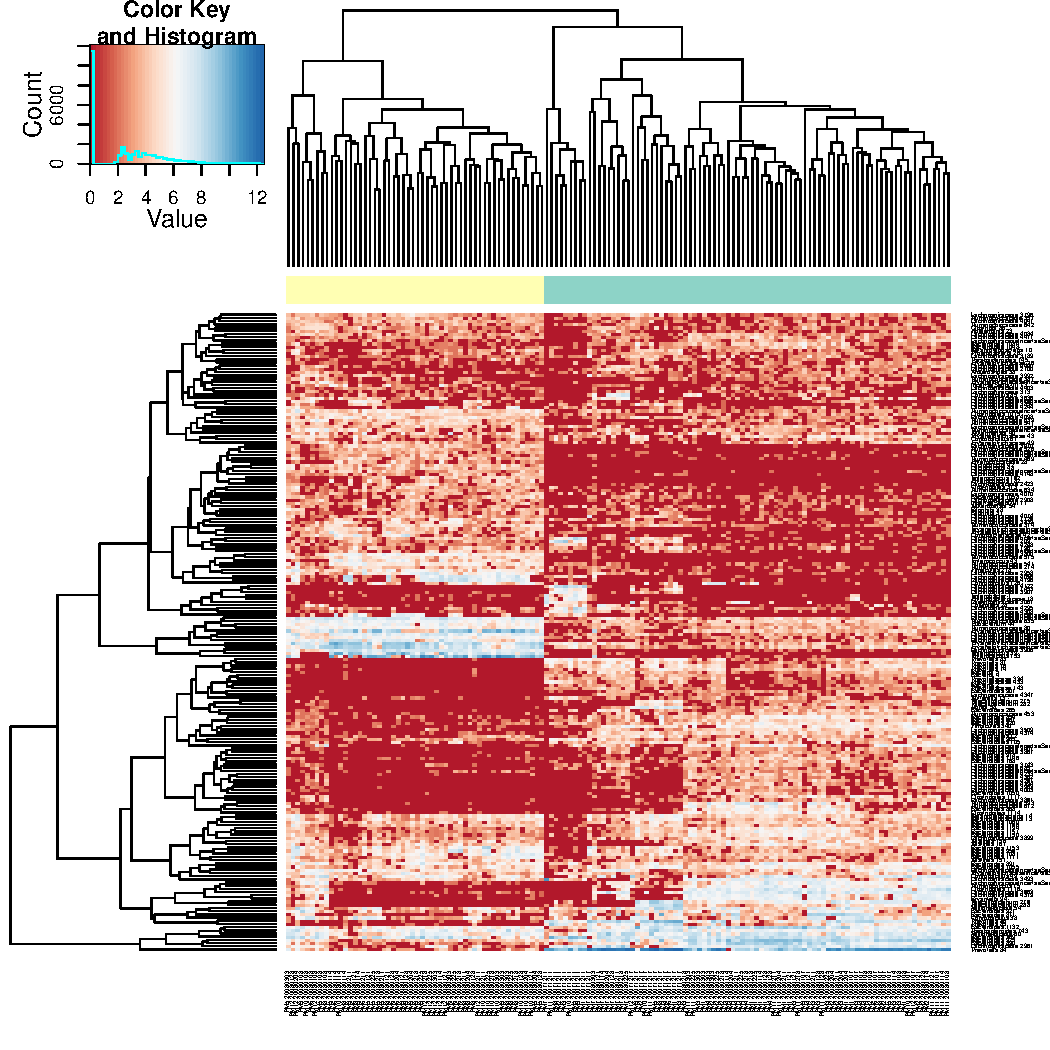
\includegraphics[width=.5\linewidth,height=.5\linewidth]{figure/heatmapData1} 
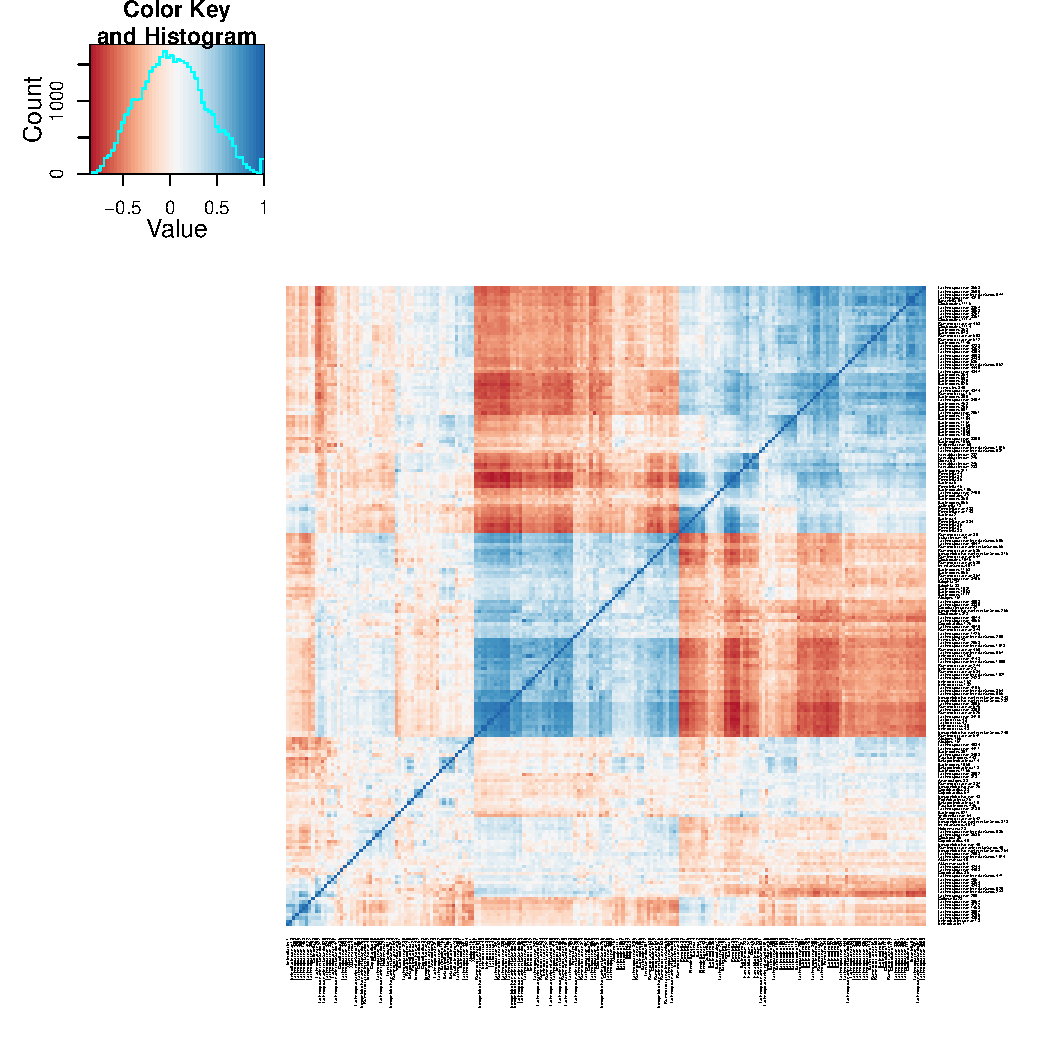
\includegraphics[width=.5\linewidth,height=.5\linewidth]{figure/heatmapData2} \caption[Left) Abundance heatmap (plotMRheatmap)]{Left) Abundance heatmap (plotMRheatmap). Right) Correlation heatmap (plotCorr).\label{fig:heatmapData}}
\end{figure}


\end{knitrout}


Below is an example of plotting CMDS plots of the data and the rarefaction effect at the OTU level. None of the data is removed (we recommend removing outliers typically).
\begin{knitrout}
\definecolor{shadecolor}{rgb}{0.969, 0.969, 0.969}\color{fgcolor}\begin{kframe}
\begin{alltt}
\hlkwd{data}\hlstd{(mouseData)}
\hlstd{cl} \hlkwb{=} \hlkwd{factor}\hlstd{(}\hlkwd{pData}\hlstd{(mouseData)}\hlopt{$}\hlstd{diet)}

\hlcom{# plotOrd - can load vegan and set distfun = vegdist and use}
\hlcom{# dist.method='bray'}
\hlkwd{plotOrd}\hlstd{(mouseData,} \hlkwc{tran} \hlstd{=} \hlnum{TRUE}\hlstd{,} \hlkwc{usePCA} \hlstd{=} \hlnum{FALSE}\hlstd{,} \hlkwc{useDist} \hlstd{=} \hlnum{TRUE}\hlstd{,} \hlkwc{bg} \hlstd{= cl,}
    \hlkwc{pch} \hlstd{=} \hlnum{21}\hlstd{,} \hlkwc{xlab} \hlstd{=} \hlstr{"1st coordinate"}\hlstd{,} \hlkwc{ylab} \hlstd{=} \hlstr{"2nd coordinate"}\hlstd{)}

\hlcom{# plotRare}
\hlstd{res} \hlkwb{=} \hlkwd{plotRare}\hlstd{(mouseData,} \hlkwc{cl} \hlstd{= cl,} \hlkwc{ret} \hlstd{=} \hlnum{TRUE}\hlstd{,} \hlkwc{pch} \hlstd{=} \hlnum{21}\hlstd{,} \hlkwc{bg} \hlstd{= cl)}

\hlcom{# Linear fits for plotRare / legend}
\hlstd{tmp} \hlkwb{=} \hlkwd{lapply}\hlstd{(}\hlkwd{levels}\hlstd{(cl),} \hlkwa{function}\hlstd{(}\hlkwc{lv}\hlstd{)} \hlkwd{lm}\hlstd{(res[,} \hlstr{"ident"}\hlstd{]} \hlopt{~} \hlstd{res[,} \hlstr{"libSize"}\hlstd{]} \hlopt{-}
    \hlnum{1}\hlstd{,} \hlkwc{subset} \hlstd{= cl} \hlopt{==} \hlstd{lv))}
\hlkwa{for} \hlstd{(i} \hlkwa{in} \hlnum{1}\hlopt{:}\hlkwd{length}\hlstd{(}\hlkwd{levels}\hlstd{(cl))) \{}
    \hlkwd{abline}\hlstd{(tmp[[i]],} \hlkwc{col} \hlstd{= i)}
\hlstd{\}}
\hlkwd{legend}\hlstd{(}\hlstr{"topleft"}\hlstd{,} \hlkwd{c}\hlstd{(}\hlstr{"Diet 1"}\hlstd{,} \hlstr{"Diet 2"}\hlstd{),} \hlkwc{text.col} \hlstd{=} \hlkwd{c}\hlstd{(}\hlnum{1}\hlstd{,} \hlnum{2}\hlstd{),} \hlkwc{box.col} \hlstd{=} \hlnum{NA}\hlstd{)}
\end{alltt}
\end{kframe}\begin{figure}[]

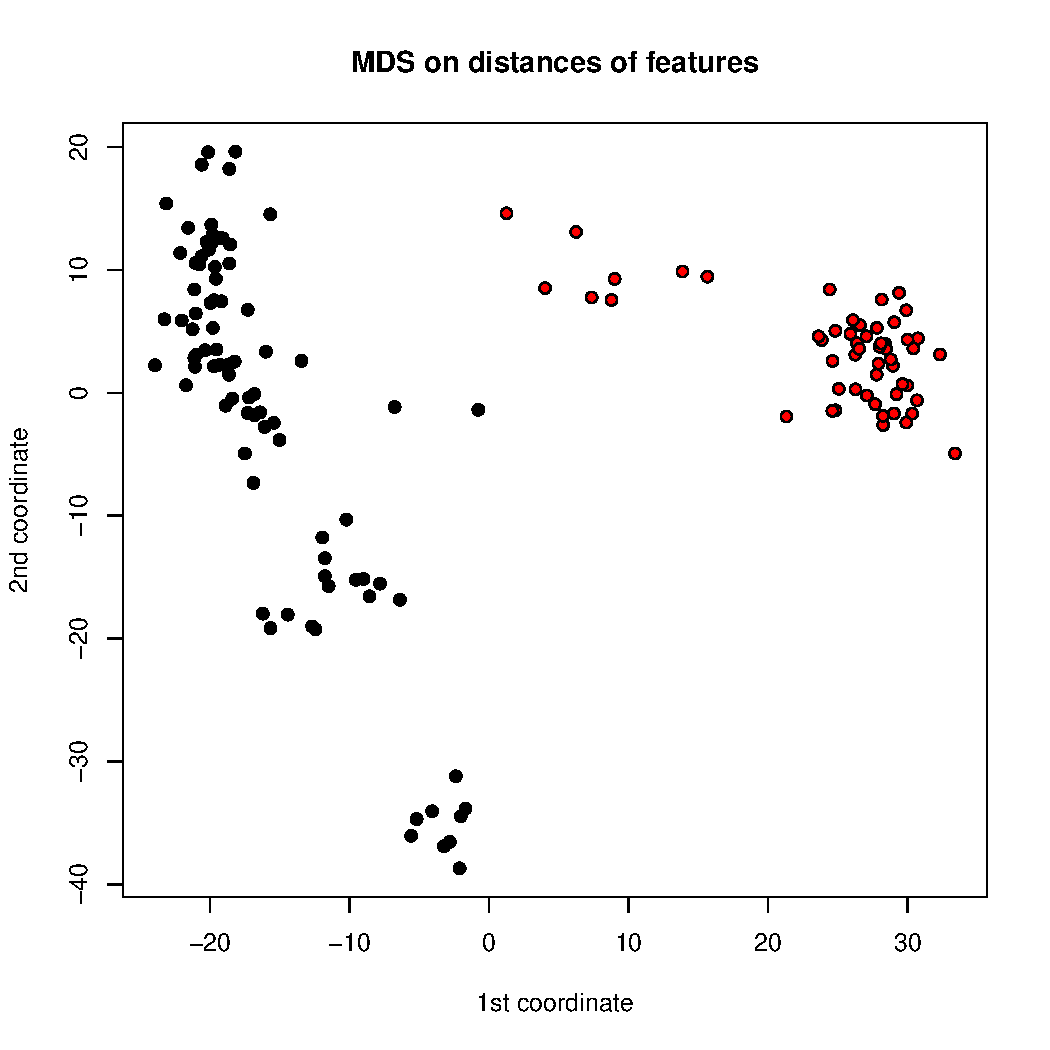
\includegraphics[width=.5\linewidth,height=.5\linewidth]{figure/MDSandRareplots1} 
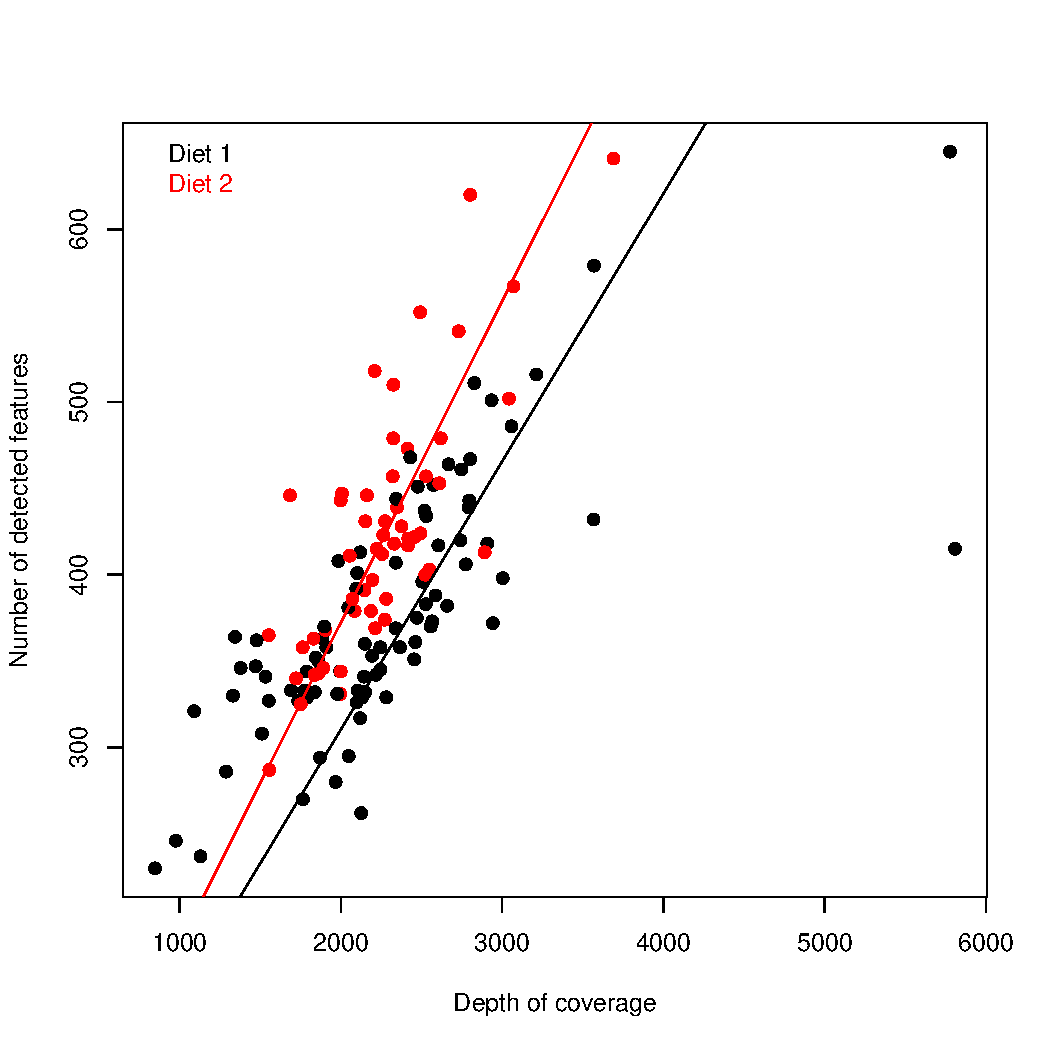
\includegraphics[width=.5\linewidth,height=.5\linewidth]{figure/MDSandRareplots2} \caption[Left) CMDS of features (plotOrd)]{Left) CMDS of features (plotOrd). Right) Rarefaction effect (plotRare).\label{fig:MDSandRareplots}}
\end{figure}


\end{knitrout}


\subsection{Feature specific}
Reads clustered with high similarity represent functional or taxonomic units. 
However, it is possible that reads from the same organism get clustered into
multiple OTUs. Following differential abundance analysis. 
It is important to confirm differential abundance. 
One way to limit false positives is ensure that the feature is actually abundant (enough positive samples). 
Another way is to plot the abundances of features similarly annotated.

\begin{enumerate}
\item \texttt{plotOTU} - abundances of a particular feature by group (Fig. 6 left)
\item \texttt{plotGenus} - abundances for several features similarly annotated by group (Fig. 6 right)
\end{enumerate}


Below we use \texttt{plotOTU} to plot the normalized log(cpt) of a specific OTU annotated as \textit{Neisseria meningitidis}, in particular the 779th row of lungTrim's count matrix. Using \texttt{plotGenus} we plot the normalized log(cpt) of all OTUs annotated as \textit{Neisseria meningitidis}. 

It would appear that \textit{Neisseria meningitidis} is differentially more abundant in nonsmokers.
\begin{knitrout}
\definecolor{shadecolor}{rgb}{0.969, 0.969, 0.969}\color{fgcolor}\begin{kframe}
\begin{alltt}
\hlkwd{head}\hlstd{(}\hlkwd{MRtable}\hlstd{(fit,} \hlkwc{coef} \hlstd{=} \hlnum{2}\hlstd{,} \hlkwc{taxa} \hlstd{=} \hlnum{1}\hlopt{:}\hlkwd{length}\hlstd{(}\hlkwd{fData}\hlstd{(lungTrim)}\hlopt{$}\hlstd{taxa)))}
\end{alltt}
\begin{verbatim}
##     +samples in group 1 +samples in group 0 counts in group 1
## 63                    6                  24                11
## 779                   7                  23                22
## 358                   1                  24                 1
## 25                   26                  15              1893
## 499                   2                  21                 2
## 21                   23                  14              1447
##     counts in group 0 smokingStatusSmoker    pValue adjPvalue
## 63               1538              -4.130 2.138e-15 1.467e-13
## 779              1512              -3.992 2.056e-14 1.113e-12
## 358               390              -2.859 9.189e-12 2.781e-10
## 25                162               2.698 6.764e-09 6.609e-08
## 499               326              -2.696 9.323e-10 1.411e-08
## 21                331               2.646 1.297e-10 2.696e-09
\end{verbatim}
\begin{alltt}
\hlstd{patients} \hlkwb{=} \hlkwd{sapply}\hlstd{(}\hlkwd{strsplit}\hlstd{(}\hlkwd{rownames}\hlstd{(}\hlkwd{pData}\hlstd{(lungTrim)),} \hlkwc{split} \hlstd{=} \hlstr{"_"}\hlstd{),}
    \hlkwa{function}\hlstd{(}\hlkwc{i}\hlstd{) \{}
        \hlstd{i[}\hlnum{3}\hlstd{]}
    \hlstd{\})}
\hlkwd{pData}\hlstd{(lungTrim)}\hlopt{$}\hlstd{patients} \hlkwb{=} \hlstd{patients}
\hlstd{classIndex} \hlkwb{=} \hlkwd{list}\hlstd{(}\hlkwc{smoker} \hlstd{=} \hlkwd{which}\hlstd{(}\hlkwd{pData}\hlstd{(lungTrim)}\hlopt{$}\hlstd{SmokingStatus} \hlopt{==}
    \hlstr{"Smoker"}\hlstd{))}
\hlstd{classIndex}\hlopt{$}\hlstd{nonsmoker} \hlkwb{=} \hlkwd{which}\hlstd{(}\hlkwd{pData}\hlstd{(lungTrim)}\hlopt{$}\hlstd{SmokingStatus} \hlopt{==} \hlstr{"NonSmoker"}\hlstd{)}
\hlstd{otu} \hlkwb{=} \hlnum{779}

\hlcom{# plotOTU}
\hlkwd{plotOTU}\hlstd{(lungTrim,} \hlkwc{otu} \hlstd{= otu, classIndex,} \hlkwc{main} \hlstd{=} \hlstr{"Neisseria meningitidis"}\hlstd{)}

\hlcom{# Now multiple OTUs annotated similarly}
\hlstd{x} \hlkwb{=} \hlkwd{fData}\hlstd{(lungTrim)}\hlopt{$}\hlstd{taxa[otu]}
\hlstd{otulist} \hlkwb{=} \hlkwd{grep}\hlstd{(x,} \hlkwd{fData}\hlstd{(lungTrim)}\hlopt{$}\hlstd{taxa)}

\hlcom{# plotGenus}
\hlkwd{plotGenus}\hlstd{(lungTrim, otulist, classIndex,} \hlkwc{labs} \hlstd{=} \hlnum{FALSE}\hlstd{,} \hlkwc{main} \hlstd{=} \hlstr{"Neisseria meningitidis"}\hlstd{)}

\hlstd{lablist} \hlkwb{<-} \hlkwd{c}\hlstd{(}\hlstr{"S"}\hlstd{,} \hlstr{"NS"}\hlstd{)}
\hlkwd{axis}\hlstd{(}\hlnum{1}\hlstd{,} \hlkwc{at} \hlstd{=} \hlkwd{seq}\hlstd{(}\hlnum{1}\hlstd{,} \hlnum{6}\hlstd{,} \hlkwc{by} \hlstd{=} \hlnum{1}\hlstd{),} \hlkwc{labels} \hlstd{=} \hlkwd{rep}\hlstd{(lablist,} \hlkwc{times} \hlstd{=} \hlnum{3}\hlstd{))}
\end{alltt}
\end{kframe}\begin{figure}[]

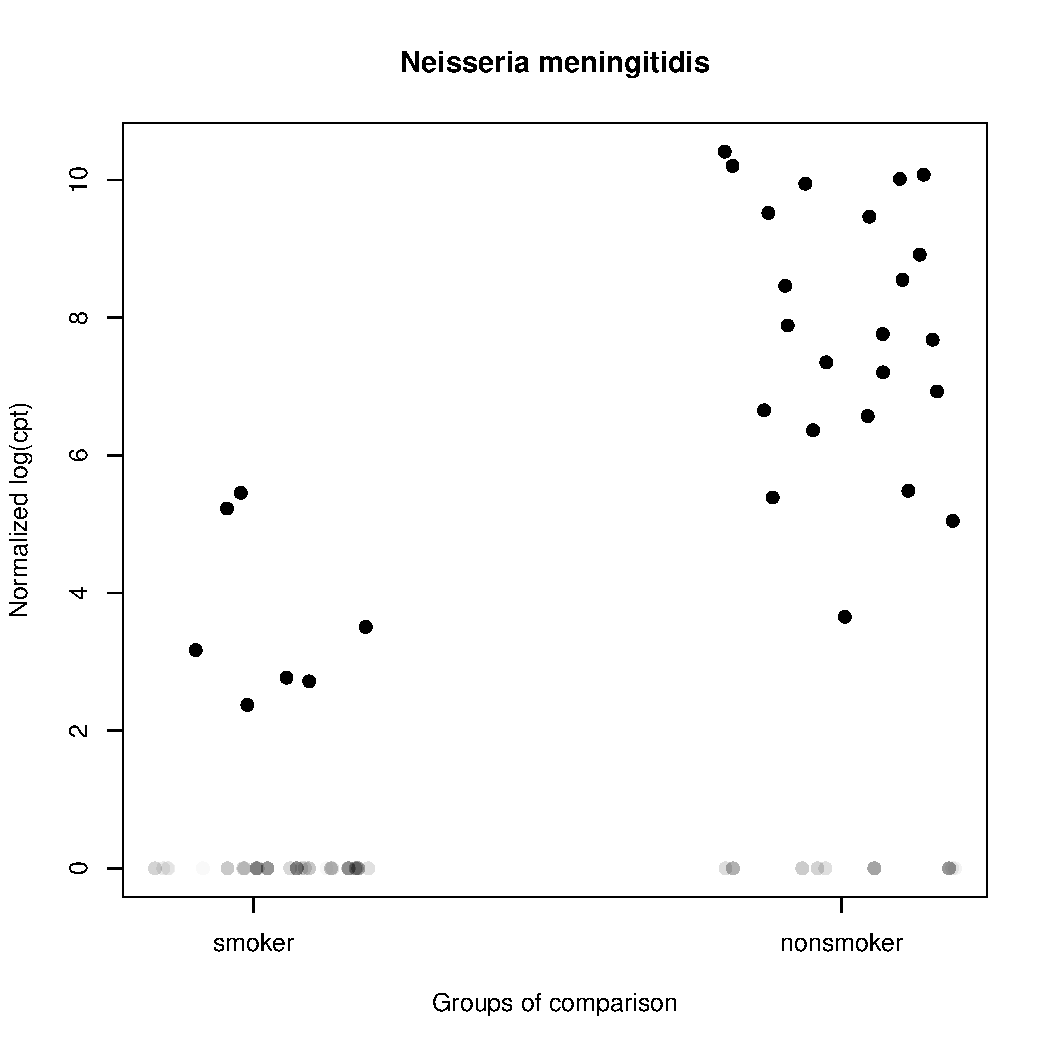
\includegraphics[width=.5\linewidth,height=.5\linewidth]{figure/plotOTUData1} 
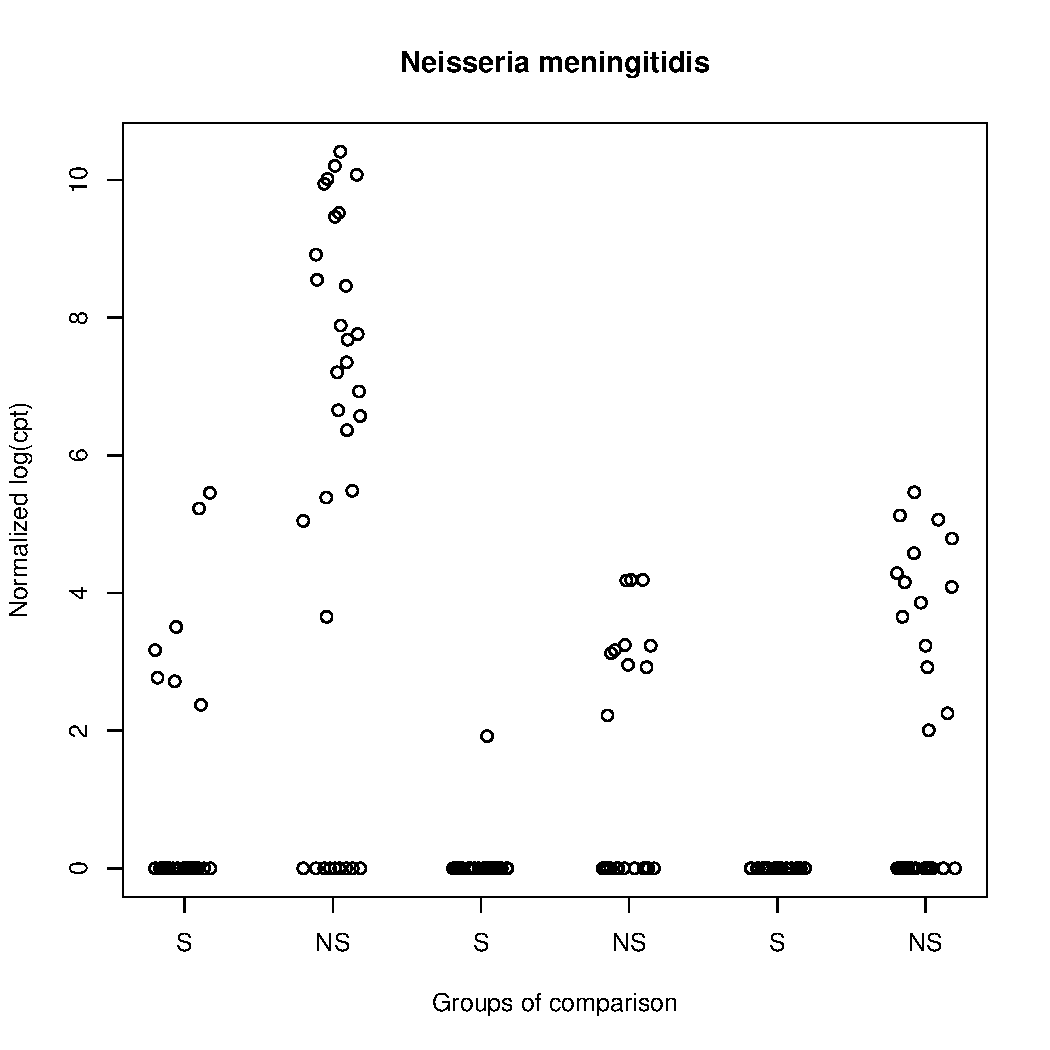
\includegraphics[width=.5\linewidth,height=.5\linewidth]{figure/plotOTUData2} \caption[Left) Abundance plot (plotOTU)]{Left) Abundance plot (plotOTU). Right) Multiple OTU abundances (plotGenus).\label{fig:plotOTUData}}
\end{figure}


\end{knitrout}


\newpage
\section{Summary}

\texttt{metagenomeSeq} is specifically designed for sparse high-throughput sequencing experiments that addresses the analysis of differential abundance for marker gene survey data. The package, while designed for marker-gene survey datasets, may be appropriate for other sparse data sets for which the zero-inflated Gaussian mixture model may apply. If you make use of the statistical method please cite our paper. If you made use of the manual/software, please cite the manual/software!

\subsection{Citing metagenomeSeq}
\begin{knitrout}
\definecolor{shadecolor}{rgb}{0.969, 0.969, 0.969}\color{fgcolor}\begin{kframe}
\begin{alltt}
\hlkwd{citation}\hlstd{(}\hlstr{"metagenomeSeq"}\hlstd{)}
\end{alltt}
\begin{verbatim}
## 
## Please cite the top for the original statistical method
## and normalization method implemented in metagenomeSeq and
## the bottom for the software/vignette guide.
## 
##   JN Paulson, OC Stine, HC Bravo, M Pop.  Differential
##   abundance analysis for microbial marker-gene surveys.
##   Nat Meth Accepted
## 
##   JN Paulson, M Pop, HC Bravo. metagenomeSeq: Statistical
##   analysis for sparse high-throughput sequncing.
##   Bioconductor package: 1.5.27.
##   http://cbcb.umd.edu/software/metagenomeSeq
\end{verbatim}
\end{kframe}
\end{knitrout}


\subsection{Session Info}
\begin{knitrout}
\definecolor{shadecolor}{rgb}{0.969, 0.969, 0.969}\color{fgcolor}\begin{kframe}
\begin{alltt}
\hlkwd{sessionInfo}\hlstd{()}
\end{alltt}
\begin{verbatim}
## R version 3.0.2 (2013-09-25)
## Platform: x86_64-apple-darwin10.8.0 (64-bit)
## 
## locale:
## [1] en_US.UTF-8/en_US.UTF-8/en_US.UTF-8/C/en_US.UTF-8/en_US.UTF-8
## 
## attached base packages:
## [1] parallel  stats     graphics  grDevices utils     datasets 
## [7] methods   base     
## 
## other attached packages:
## [1] metagenomeSeq_1.5.27 gplots_2.12.1       
## [3] RColorBrewer_1.0-5   matrixStats_0.8.12  
## [5] limma_3.18.4         Biobase_2.22.0      
## [7] BiocGenerics_0.8.0   knitr_1.5           
## 
## loaded via a namespace (and not attached):
##  [1] bitops_1.0-6       caTools_1.16       evaluate_0.5.1    
##  [4] formatR_0.10       gdata_2.13.2       gtools_3.1.1      
##  [7] highr_0.3          KernSmooth_2.23-10 R.methodsS3_1.5.2 
## [10] stringr_0.6.2      tools_3.0.2
\end{verbatim}
\end{kframe}
\end{knitrout}


\newpage
\section{Appendix}
\subsection{Appendix A: MRexperiment internals}
The S4 class system in R allows for object oriented definitions. \texttt{metagenomeSeq} makes use of the \texttt{Biobase} package in Bioconductor and their virtual-class, \texttt{eSet}. Building off of \texttt{eSet}, the main S4 class in \texttt{metagenomeSeq} is termed \texttt{MRexperiment}. \texttt{MRexperiment} is a simple extension of \texttt{eSet}, adding a single slot, \texttt{expSummary}.

The experiment summary slot is a data frame that includes the depth of coverage and the normalization factors for each sample. Future datasets can be formated as MRexperiment objects and analyzed with relative ease. A \texttt{MRexperiment} object is created by calling \texttt{newMRexperiment}, passing the counts, phenotype and feature data as parameters.

We do not include normalization factors or library size in the currently available slot specified for the sample specific phenotype data. All matrices are organized in the \texttt{assayData} slot. All phenotype data (disease status, age, etc.) is stored in \texttt{phenoData} and feature data (OTUs, taxanomic assignment to varying levels, etc.) in \texttt{featureData}. Additional slots are available for reproducibility and annotation.

\subsection{Appendix B: Mathematical model}

Defining the class comparison of interest as $k(j)=I\{j \in \mathrm{ group } A\}$. The zero-inflated model is defined for the continuity-corrected $\log_2$ of the count data $y_{ij} = \log_2(c_{ij}+1)$ as a mixture of a point mass at zero $I_{\{0\}}(y_{ij})$ and a count distribution $f_{count}(y_{ij};\mu_i, \sigma_i^2) \sim N(\mu_i, \sigma_i^2)$.
Given mixture parameters $\pi_{j}$, we have that the density of the zero-inflated Gaussian distribution for feature $i$, in sample $j$ with $S_{j}$ total counts is:

\begin{equation}
f_{zig}(y_{ij}; \theta ) = \pi_{j}(S_{j}) \cdot I_{\{0\}}(y_{ij})
+ (1-\pi_{j}(S_{j})) \cdot f_{count}(y_{ij};\theta)
\end{equation}

Maximum-likelihood estimates are approximated using an EM algorithm,
where we treat mixture membership $\Delta_{ij}=1$ if $y_{ij}$ is
generated from the zero point mass as latent indicator variables\cite{EM}. We make use of an EM algorithm to account for the linear relationship between sparsity and depth of coverage. The user can specify within the \texttt{fitZig} function a non-default zero model that accounts for more than simply the depth of coverage (e.g. country, age, any metadata associated with sparsity, etc.).
See Figure 7 for the graphical model.

\begin{figure}
\centerline{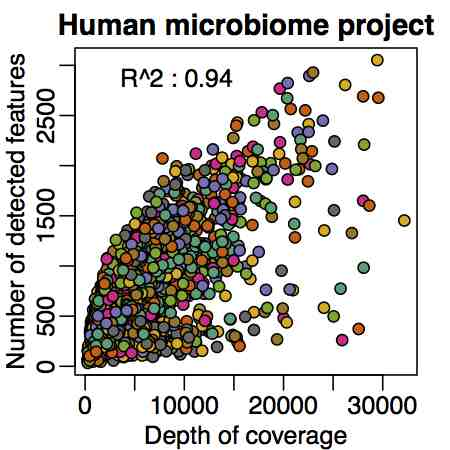
\includegraphics[width=.7\textwidth]{metagenomeSeq_figure2.png}}
\caption{\footnotesize{Graphical model. Green nodes represent observed variables: $S_j$ is the
total number of reads in sample $j$; $k_j$ the case-control status
of sample $j$; and $y_{ij}$ the logged normalized counts for feature $i$ in sample $j$. Yellow nodes represent counts obtained from each mixture component: counts come from either a spike-mass at zero,
$y_{ij}^0$, or the ``count'' distribution, $y_{ij}^1$. Grey nodes $b_{0i}$, $b_{1i}$ and $\sigma_{i}^2$ represent the
estimated overall mean, fold-change and variance of the count distribution component for feature $i$. $\pi_j$, is the mixture proportion for sample $j$ which depends on sequencing depth via a linear model defined by parameters $\beta_0$ and $\beta_1$. The expected value of latent indicator variables $\Delta_{ij}$ give the posterior  probability of a count being generated from a spike-mass at zero, i.e. $y_{ij}^0$. We assume $M$ features and $N$ samples.}}
\end{figure}

More information will be included later.  For now, please see the online methods in: 

http://www.nature.com/nmeth/journal/vaop/ncurrent/full/nmeth.2658.html

\subsection{Appendix C: Calculating the proper percentile} To be included: an overview of the two methods implemented for the data driven percentile calculation and more description below.


The choice of the appropriate quantile given is crucial for ensuring that the normalization approach does not introduce normalization-related artifacts in the data. At a high level, the count distribution of samples should all be roughly equivalent and independent of each other up to this quantile under the assumption that, at this range, counts are derived from a common distribution.


More information will be included later. For now, please see the online methods in: 

http://www.nature.com/nmeth/journal/vaop/ncurrent/full/nmeth.2658.html

\newpage
\bibliography{metagenomeSeq}
\end{document}
